\chapter{薄内层怎样选出增长率：从标度到匹配常数}\label{tm:matching}
\section{先列近似，再删项}
本章取$\gamma>0$、$\Delta'>0$的经典撕裂支。近共振面，$F=B_{0y}\simeq B'_0x$，Harris片有$B'_0=B_0/a$。假设内层$|x|\sim\delta\ll a$，同时$k\delta\ll1$。在适当薄层排序下，$k^2\Psi$小于横向二阶导数，$F''\Psi$小于$F\Psi''$；但$D_\eta\Psi''$与惯性$\gamma\Phi''$不能再删。式\eqref{tm:realind}--\eqref{tm:realvort}约化为
\begin{align}
 \gamma\Psi&=kB'_0x\Phi+D_\eta\Psi'',\label{tm:inner1}\\
 \gamma\Phi''&=-\frac{kB'_0}{\mu_0\rho}x\Psi''.
 \label{tm:inner2}
\end{align}
必须同时求解两条式子。只用“扩散时间等于增长时间”会漏掉磁张力和流体惯性，因此得不到FKR的$3/5$指数。

下面把$X=x/a$、$K=ka$、$\epsilon=\delta/a$、$\hat\gamma=\gamma a/V_A$、$\Delta=\Delta'a$作为简记。磁通和流函数分别按$B_0a$、$V_Aa$归一化，两条内层方程成为
\begin{align}
 \hat\gamma\Psi&=KX\Phi+S_a^{-1}\Psi_{XX},\label{tm:innernorm1}\\
 \hat\gamma\Phi_{XX}&=-KX\Psi_{XX}.
 \label{tm:innernorm2}
\end{align}
这里为便于阅读，$\Psi,\Phi$暂省去归一化帽号，但导数明确写成$XX$。有量纲公式会重新标出。

\section{常磁通近似并不是磁场不变}
设内层跨越时磁通扰动仅有小变化：$\Psi(X)=\Psi_s+\psi_c(X)$，$|\psi_c|\ll|\Psi_s|$。由外区匹配，导数跳跃为$\Delta\Psi_s$，而跳跃发生在尺度$\epsilon$内，因此
\begin{equation}
 \Psi_{XX}\sim\frac{\Delta\Psi_s}{\epsilon},\qquad
 \psi_c\sim\Psi_{XX}\epsilon^2\sim\Delta\epsilon\Psi_s.
 \label{tm:constpsiscaling}
\end{equation}
所以常磁通（constant-$\psi$）条件是
\begin{equation}
 \boxed{\Delta'\delta=\Delta\epsilon\ll1.}
 \label{tm:constpsicond}
\end{equation}
它表示\emph{磁通扰动振幅}在层内近似常数。它并不表示$\Psi'=0$、电流为零或没有重联。微小变化除以微小层宽后，二阶导数仍可很大。

一个数值类比：取归一化磁通变化$\psi_c/\Psi_s=0.01$、层宽$\epsilon=0.005$，则$\Psi_{XX}/\Psi_s\sim0.01/(0.005)^2=400$。函数值只变1\%，二阶导数却达到400；在内层保留电阻项毫不矛盾。

\section{FKR标度：三个平衡，逐步消去未知量}
由涡量式\eqref{tm:innernorm2}，取$X\sim\epsilon$、$\Phi_{XX}\sim\Phi/\epsilon^2$并使用式\eqref{tm:constpsiscaling}，得到
\begin{equation}
 \hat\gamma\frac{\Phi}{\epsilon^2}
 \sim K\epsilon\frac{\Delta\Psi_s}{\epsilon}
 =K\Delta\Psi_s.
\end{equation}
因此
\begin{equation}
 \Phi\sim\frac{K\Delta\epsilon^2}{\hat\gamma}\Psi_s.
 \label{tm:phiscale}
\end{equation}
磁通式中的时间项、电阻项与平流项共同参与主阶平衡。时间与电阻比较：
\begin{equation}
 \hat\gamma\Psi_s\sim S_a^{-1}\frac{\Delta\Psi_s}{\epsilon}
 \quad\Rightarrow\quad
 \hat\gamma\sim S_a^{-1}\frac{\Delta}{\epsilon}.
 \label{tm:resbalance}
\end{equation}
时间与平流比较，并代入式\eqref{tm:phiscale}：
\begin{equation}
 \hat\gamma\Psi_s\sim K\epsilon\Phi
 \sim\frac{K^2\Delta\epsilon^3}{\hat\gamma}\Psi_s
 \quad\Rightarrow\quad
 \hat\gamma^2\sim K^2\Delta\epsilon^3.
 \label{tm:advbalance}
\end{equation}
把式\eqref{tm:resbalance}平方，代入式\eqref{tm:advbalance}：
\begin{align}
 S_a^{-2}\frac{\Delta^2}{\epsilon^2}&\sim K^2\Delta\epsilon^3,\\
 \epsilon^5&\sim S_a^{-2}\Delta K^{-2},\\
 \boxed{\epsilon\sim S_a^{-2/5}\Delta^{1/5}K^{-2/5}.}\label{tm:FKRdelta}
\end{align}
再代回$\hat\gamma\sim S_a^{-1}\Delta/\epsilon$，逐个合并幂指数：
\begin{equation}
 \boxed{\hat\gamma\sim
 S_a^{-1+2/5}\Delta^{1-1/5}K^{2/5}
 =S_a^{-3/5}\Delta^{4/5}K^{2/5}.}
 \label{tm:FKRgamma}
\end{equation}
这就是经典常磁通电阻撕裂标度。$\gamma\propto D_\eta^{3/5}$说明电阻趋零时，在\emph{固定厚度、固定波数、固定外区驱动}条件下增长率趋零。后面薄片的厚度本身随$S$变化时，不能沿用这个“固定几何”的解释。

\paragraph{回查刚才删掉的$k^2$项。}
在常磁通层内，$k^2\Psi/\Psi''\sim K^2\epsilon/\Delta$。通常远离$\Delta=0$且层很薄时满足小量；但靠近边际$K\to1$，$\Delta$很小，不能只凭$k\delta\ll1$就保证所有删项。FKR公式在严格边际附近与更高阶效应的次序，应重新核对，而非任意精确外推到$\Delta=0$附近。

\section{再前进一步：常磁通匹配系数不是随意拟合}
上节的$\sim$没有决定$O(1)$系数。本节给出其来源；若首次阅读不熟悉特殊函数，可以先掌握式\eqref{tm:FKRexact}，随后沿下面的步骤复算。这里的数学稍深，但没有增加新的物理假设。

回到有量纲式\eqref{tm:inner1}，在时间项中取$\Psi\simeq\Psi_s$，但\emph{仍保留}$\Psi''$。定义
\begin{equation}
 \delta_*\equiv\left[\frac{\mu_0\rho D_\eta\gamma}{k^2(B'_0)^2}\right]^{1/4},
 \quad \xi=\frac{x}{\delta_*},\quad
 \Phi(x)=\frac{\gamma\Psi_s}{kB'_0\delta_*}\,f(\xi).
 \label{tm:deltastar}
\end{equation}
$\delta_*$是一种明确的内层特征尺度，不是电流半高全宽；不同论文对“层宽”的定义会给不同数值系数。由磁通式直接得到
\begin{equation}
 \Psi''=\frac{\gamma\Psi_s}{D_\eta}[1-\xi f(\xi)].
 \label{tm:psisecond}
\end{equation}
再将它与$\Phi''=\gamma\Psi_s f''/(kB'_0\delta_*^3)$代入涡量式，除去公共系数：
\begin{equation}
 f''=-\frac{k^2(B'_0)^2\delta_*^4}{\mu_0\rho D_\eta\gamma}\,\xi(1-\xi f)
 =-\xi(1-\xi f).
\end{equation}
所以需要求解的\emph{无参数}内层形状方程是
\begin{equation}
 \boxed{f''-\xi^2f=-\xi,\qquad f(-\xi)=-f(\xi),\quad
 f(\xi)\sim\xi^{-1}\ (|\xi|\to\infty).}
 \label{tm:shapeODE}
\end{equation}
远场条件来自理想关系$\Phi=\gamma\Psi_s/(kB'_0x)$；不是任意设定的边界条件。

将式\eqref{tm:psisecond}跨内层积分，再用式\eqref{tm:currentjump}匹配，
\begin{align}
 \Delta'\Psi_s&=\frac{\gamma\Psi_s\delta_*}{D_\eta}
 \int_{-\infty}^{\infty}[1-\xi f(\xi)]\,\dd\xi,\\
 \Delta'&=I\frac{\gamma\delta_*}{D_\eta},\qquad
 I\equiv\int_{-\infty}^{\infty}[1-\xi f(\xi)]\,\dd\xi.
 \label{tm:matchI}
\end{align}
$\Psi_s$完全约去，所以线性增长率不依赖任意选择的小种子振幅。种子影响需要等待多久才达到非线性幅度，却不改变这里的本征增长率。

\subsection{通过正弦变换求\texorpdfstring{$I$}{I}}
令$\mathcal F(p)=\int_0^\infty f(\xi)\sin(p\xi)\,\dd\xi$，其中$p>0$是\emph{内层坐标}$\xi$的变换变量，和沿片波数$k$不同。积分可先乘$e^{-\varepsilon\xi}$，计算后令$\varepsilon\to0^+$，以正确处理$f\sim1/\xi$的远场。

两次分部积分给$\int f''\sin(p\xi)\dd\xi=-p^2\mathcal F$，而对$p$两次求导给$\int\xi^2f\sin(p\xi)\dd\xi=-\mathcal F''$。式\eqref{tm:shapeODE}右端$-\xi$的带阻尼变换在固定$p>0$后取极限为零，故
\begin{equation}
 \mathcal F''-p^2\mathcal F=0\quad(p>0).
\end{equation}
远场$f\sim1/\xi$决定$\mathcal F(0^+)=\pi/2$。这个值可以从
$\int_0^\infty e^{-\varepsilon\xi}\sin(p\xi)\dd\xi/\xi
=\arctan(p/\varepsilon)$看出；在$\varepsilon\to0^+$后得到$\pi/2$。还要求$\mathcal F(p)$在$p\to\infty$衰减。

令$z=p^2/2$、$\mathcal F=\sqrt p\,H(z)$。为避免跳过链式法则，这里把两次求导写开（$H'$对$z$求导）：
\begin{align*}
 \mathcal F'&=\frac{H}{2\sqrt p}+p^{3/2}H',\\
 \mathcal F''&=-\frac{H}{4p^{3/2}}+2p^{1/2}H'+p^{5/2}H''.
\end{align*}
将$\mathcal F''-p^2\mathcal F=0$除以$p^{5/2}$得
$H''+(2/p^2)H'-(1+1/(4p^4))H=0$。再用$p^2=2z$并乘$z^2$，得到
\begin{equation}
 z^2H''+zH'-(z^2+1/16)H=0.
\end{equation}
这是阶数$1/4$的修正Bessel方程；其衰减解记为$K_{1/4}(z)$。它可以用积分定义：
\begin{equation*}
 K_\nu(z)=\int_0^\infty e^{-z\cosh t}\cosh(\nu t)\dd t.
\end{equation*}
它只是上述微分方程的函数解，并非另外一个物理模型。因此
\begin{equation}
 \mathcal F(p)=C\sqrt p\,K_{1/4}(p^2/2).
\end{equation}
在$p\to0^+$，由此函数的两个独立小参数幂解，
\begin{equation}
 \sqrt p\,K_{1/4}(p^2/2)
 =\frac{\Gamma(1/4)}{\sqrt2}
 +\frac{\Gamma(-1/4)}{2\sqrt2}\,p+O(p^4).
\end{equation}
$\Gamma$是Gamma函数，$\Gamma(s)=\int_0^\infty t^{s-1}e^{-t}\dd t$（先取$s>0$，其余用递推延拓）。分部积分给$\Gamma(s+1)=s\Gamma(s)$，故$\Gamma(-1/4)=-4\Gamma(3/4)$。归一化$\mathcal F(0^+)=\pi/2$后，
\begin{equation}
 \mathcal F'(0^+)=-\pi\frac{\Gamma(3/4)}{\Gamma(1/4)}.
\end{equation}
由于$1-\xi f$为偶函数，且其半轴余弦变换在$p>0$为$-\mathcal F'(p)$，令$p\to0^+$便得到
\begin{equation}
 \boxed{I=-2\mathcal F'(0^+)
 =2\pi\frac{\Gamma(3/4)}{\Gamma(1/4)}=2.12364827.}
\end{equation}
这里对常数1的变换也要使用同一阻尼极限；不能把两个分别不收敛的积分先随意拆开，再分别令$p=0$。

\subsection{解出含系数的增长率}
把式\eqref{tm:deltastar}代入式\eqref{tm:matchI}：
\begin{equation}
 \Delta'=I\gamma^{5/4}D_\eta^{-3/4}
 \left(\frac{kB'_0}{\sqrt{\mu_0\rho}}\right)^{-1/2}.
\end{equation}
两边乘相应系数再取$4/5$次方，得
\begin{equation}
 \gamma=I^{-4/5}D_\eta^{3/5}
 \left(\frac{kB'_0}{\sqrt{\mu_0\rho}}\right)^{2/5}(\Delta')^{4/5}.
\end{equation}
对于$B'_0=B_0/a$，无量纲形式为
\begin{align}
 \boxed{\gamma\tau_A=C_\gamma S_a^{-3/5}K^{2/5}\Delta^{4/5},\quad
 C_\gamma=I^{-4/5}=0.547436725,}\label{tm:FKRexact}\\
 \frac{\delta_*}{a}=C_\delta S_a^{-2/5}K^{-2/5}\Delta^{1/5},\quad
 C_\delta=I^{-1/5}=0.860168397.
 \label{tm:FKRwidthexact}
\end{align}
这些系数属于本章无黏性、常磁通、局部线性剪切与明确宽度定义；改变闭合或层宽定义时，不应坚持使用同一个数值系数。经典FKR关系的物理来源与现代匹配写法见原始文献及作者讲义。\citep{TMFKR1963,TMFitzMatching}

\section{大\texorpdfstring{$\Delta'$}{Delta prime}：为什么必须换一套估计}
如果算出$\Delta'\delta\gtrsim1$，磁通在层内不能再近似不变。此时应取
\begin{equation}
 \Psi_{XX}\sim\frac{\Psi}{\epsilon^2},
\end{equation}
而不是$\Delta\Psi/\epsilon$。仍用同一两条内层方程，涡量平衡给
\begin{equation}
 \hat\gamma\frac{\Phi}{\epsilon^2}\sim K\epsilon\frac{\Psi}{\epsilon^2}
 \quad\Rightarrow\quad \Phi\sim\frac{K\epsilon}{\hat\gamma}\Psi.
\end{equation}
磁通的时间和平流项平衡给
$\hat\gamma\Psi\sim K\epsilon\Phi$，所以$\hat\gamma^2\sim K^2\epsilon^2$，取增长支$\hat\gamma\sim K\epsilon$。时间与电阻平衡给$\hat\gamma\sim S_a^{-1}\epsilon^{-2}$。两者相等：
\begin{align}
 K\epsilon&\sim S_a^{-1}\epsilon^{-2},\\
 \boxed{\frac{\delta}{a}\sim S_a^{-1/3}K^{-1/3},\qquad
 \gamma\tau_A\sim S_a^{-1/3}K^{2/3}.}
 \label{tm:Coppi}
\end{align}
这通常称大$\Delta'$或Coppi型区间。增长率的主阶不再显式依赖$\Delta'$，并不意味着外区消失；外区仍负责确保驱动足够大、允许该匹配极限。这里没有给一般有限$\Delta'$色散关系的精确数值常数。图中的系数1只用于量级比较。\citep{TMLoureiro2007}

\section{两个区间在哪里相遇，为什么有最快波长}
对Harris片长波$K\ll1$，$\Delta\simeq2/K$。FKR增长率因此满足
\begin{equation}
 \hat\gamma_{\rm FKR}\sim S_a^{-3/5}K^{2/5}(K^{-1})^{4/5}
 \sim S_a^{-3/5}K^{-2/5}.
\end{equation}
在这一支上，减小$K$（加长波长）使增长变快；但大$\Delta'$支满足$\hat\gamma\sim S_a^{-1/3}K^{2/3}$，减小$K$反而变慢。最快模应在两种平衡的过渡附近，而不是$K\to0$。

用常磁通失效条件$\Delta\epsilon\sim1$，
\begin{equation}
 K^{-1}S_a^{-2/5}K^{-1/5}K^{-2/5}
 =S_a^{-2/5}K^{-8/5}\sim1,
\end{equation}
得到
\begin{equation}
 \boxed{K_*\sim S_a^{-1/4},\qquad
 \hat\gamma_*\sim S_a^{-1/2},\qquad \delta_*/a\sim S_a^{-1/4}.}
 \label{tm:fastest}
\end{equation}
这里用的是幂次关系，忽略的$O(1)$系数会移动峰值；不能把两个渐近式的交点称为已经精确求得的本征谱。若盒长不允许这个$K_*$，最快的\emph{实际允许模}还要在离散$k_m$中选择。

\begin{figure}[htbp]
\centering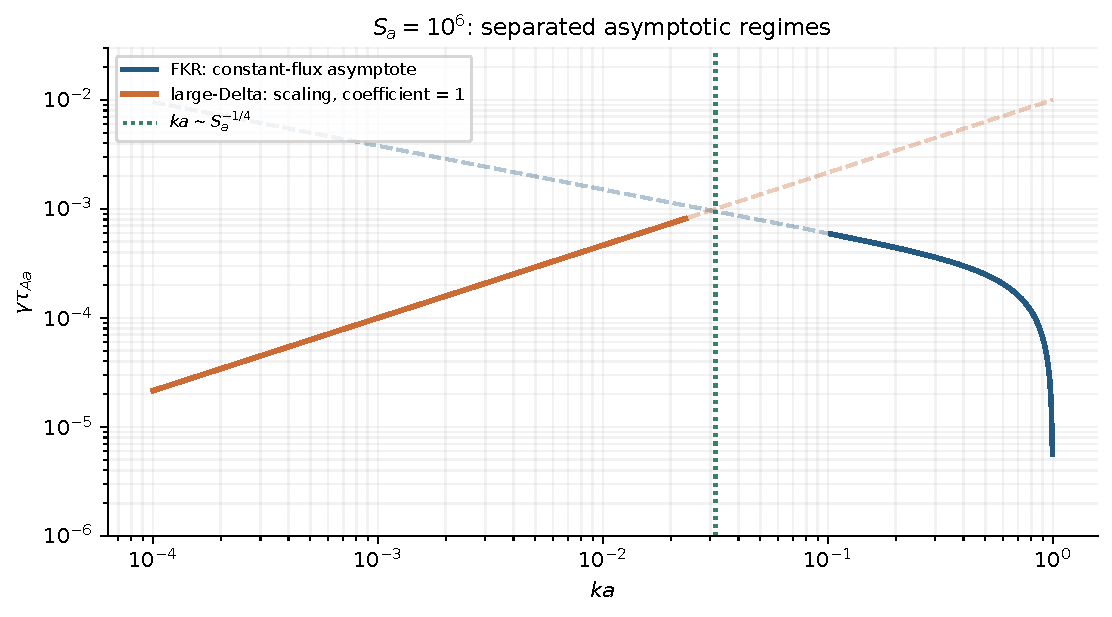
\includegraphics[width=\textwidth]{figures/tm_fkr_coppi.pdf}
\caption{$S_a=10^6$时两种渐近增长率。FKR支使用本章导出的$C_\gamma=0.5474367$；大$\Delta'$支取系数1以示量级。实线分别限制在图中所选的$\Delta'\delta<0.3$或$>3$区间，虚线是超出该条件的形式延拓；中间区域须另解完整本征问题，不能把曲线交点当精确最快模。}
\label{tm:fig:regimes}
\end{figure}

\section{完整数值算例一：得到答案后逐项检查}
本节是\textbf{自行指定系数的数学MHD教学算例}，不冒充某次实验。取
\begin{equation}
 a=0.10\,\mathrm m,\quad V_A=10^5\,\mathrm{m/s},\quad
 D_\eta=0.010\,\mathrm{m^2/s},\quad K=ka=0.50.
\end{equation}
则$\eta=\mu_0D_\eta=1.2566\times10^{-8}\,\Omega\,\mathrm m$，
\begin{align}
 S_a&=\frac{0.10\times10^5}{0.010}=10^6,\\
 \tau_A&=\frac{0.10}{10^5}=10^{-6}\,\mathrm s,\qquad
 \tau_R=\frac{(0.10)^2}{0.010}=1.0\,\mathrm s,\\
 k&=5.0\,\mathrm{m^{-1}},\quad\lambda=1.257\,\mathrm m,\quad
 \Delta=2(2-0.5)=3.
\end{align}
代入含系数FKR公式，
\begin{align}
 \gamma\tau_A&=0.5474367\,(10^6)^{-3/5}(0.5)^{2/5}3^{4/5}
 =2.50968\times10^{-4},\\
 \boxed{\gamma=250.97\,\mathrm{s^{-1}},\quad\gamma^{-1}=3.985\,\mathrm{ms}},\\
 \frac{\delta_*}{a}&=0.8601684\,(10^6)^{-2/5}(0.5)^{-2/5}3^{1/5}
 =0.00562885,\\
 \boxed{\delta_*=5.629\times10^{-4}\,\mathrm m=0.563\,\mathrm{mm}.}
\end{align}
现在检查，而不是把数字算完就结束：
\begin{align}
 \gamma\tau_A&=2.51\times10^{-4}\ll1,&\gamma\tau_R&=251\gg1,\\
 \delta_*/a&=0.00563\ll1,&k\delta_*&=0.00281\ll1,\\
 \Delta'\delta_*&=\Delta\delta_*/a=0.0169\ll1,&
 \gamma/(kV_A)&=5.02\times10^{-4}\ll1.
\end{align}
所用几何、时间、常磁通与沿片慢排序均较好满足。$k^2\Psi/\Psi''\sim K^2\epsilon/\Delta=4.69\times10^{-4}$，也很小。

无黏性还需要额外检验。如果加入运动黏度$\nu$，涡量式多出$\nu\nabla^4\phi$，内层黏性/惯性比为
\begin{equation}
 \frac{\nu\Phi/\delta_*^4}{\gamma\Phi/\delta_*^2}
 =\frac{\nu}{\gamma\delta_*^2}.
\end{equation}
本例$\gamma\delta_*^2=7.95\times10^{-5}\,\mathrm{m^2/s}$。若教学指定$\nu=10^{-6}\,\mathrm{m^2/s}$，该比值$0.0126$；若实际$\nu=10^{-2}\,\mathrm{m^2/s}$，比值约126，无黏性FKR就失效。单说“$\nu$很小”不够，必须与内层尺度比较。

\paragraph{增长率怎样对应等待时间。}
设初始岛宽$W_0=10\,\mu\mathrm m$，线性阶段$W(t)=W_0e^{\gamma t/2}$。达到$W\sim\delta_*$的时间估计为
\begin{equation}
 t_{\rm nl}\simeq\frac2\gamma\ln\frac{\delta_*}{W_0}
 =\frac2{250.97}\ln(56.29)=0.0321\,\mathrm s.
\end{equation}
此时背景扩散仍只经历约$3.2\%$的$\tau_R$。这里$W\sim\delta_*$只是非线性开启的量级判据，具体转折位置含$O(1)$定义差别；不能把0.0321秒解读成精确触发时刻。

\section{完整数值算例二：有时正确答案是旧公式不能用}
保持上节$S_a=10^6$与有量纲单位，只改变$K$。若$K=0.05$，$\Delta=39.9$。机械代入FKR得$\delta/a=0.02372$、$\gamma=791.95\,\mathrm{s^{-1}}$，但
\begin{equation}
 \Delta\delta/a=39.9\times0.02372=0.947.
\end{equation}
它不再远小于1，因此这些数字不能作为可信FKR预测；系统位于过渡区，需要解完整匹配关系或线性本征问题。

若$K=0.01$，$\Delta=199.98$，错误使用FKR会给$\Delta\delta/a=12.47$，明显不自洽。改用大$\Delta'$量级式：
\begin{align}
 \delta/a&\sim(10^6)^{-1/3}(0.01)^{-1/3}=0.04642,\\
 \gamma\tau_A&\sim(10^6)^{-1/3}(0.01)^{2/3}=4.642\times10^{-4},\\
 \delta&\sim4.64\,\mathrm{mm},\quad\gamma\sim464\,\mathrm{s^{-1}},\quad
 \gamma^{-1}\sim2.15\,\mathrm{ms},\\
 \Delta'\delta&\sim199.98\times0.04642=9.28>1.
\end{align}
这组检查支持大$\Delta'$排序，但层宽已经达到$a$的4.6\%，仍须注意渐近精度；而464这个数字只含量级系数1，不能报告为经完整本征求解的精确增长率。

若比较不同文献，必须同时记录$S_a,K,\Delta',\delta/a$、黏性与边界。只挑两组$\gamma$数字比较，很容易把不同渐近区间的差别误当成代码错误或新物理。

\section{若要数值求本征值，应求什么}
在不作内外删项时，式\eqref{tm:realind}--\eqref{tm:realvort}是关于$\Psi(x),\Phi(x),\gamma$的线性边值问题。设$\mathcal D=\dd^2/\dd x^2-k^2$，可形式化写为
\begin{equation}
 \begin{pmatrix}
 D_\eta\mathcal D&kF\\
 -k(F\mathcal D-F'')/(\mu_0\rho)&0
 \end{pmatrix}
 \begin{pmatrix}\Psi\\\Phi\end{pmatrix}
 =\gamma
 \begin{pmatrix}1&0\\0&\mathcal D\end{pmatrix}
 \begin{pmatrix}\Psi\\\Phi\end{pmatrix}.
\end{equation}
右侧第二个矩阵不等于单位阵，因为涡量包含二阶导数。无穷域可在$|x|=L_x$用远场衰减条件近似；有限壁面则必须使用相应磁通和流动边界，不应混作同一种问题。

检查至少包括：扩大$L_x$后增长率不再变化；增加内层网格后$\gamma$与电流积分收敛；$\Psi$偶、$\Phi$奇的目标奇偶性正确；内区积分给出的$\Delta'$与外区解一致；低$S$、过渡区和黏性较强时不强求吻合无黏性FKR式。\textbf{本讲义给出了可复算解析与量级计算，没有声称已运行该完整本征求解或实验复现。}
